% easychair.tex,v 3.5 2017/03/15

\documentclass{easychair}


\usepackage{doc}
%
\newcommand{\easychair}{\textsf{easychair}}
\newcommand{\miktex}{MiK{\TeX}}
\newcommand{\texniccenter}{{\TeX}nicCenter}
\newcommand{\makefile}{\texttt{Makefile}}
\newcommand{\latexeditor}{LEd}

%\makeindex

%% Front Matter
%%
% Regular title as in the article class.
%
\title{Automatic On-Chain Verification of Java Smart Contracts}

\author{
Luca Olivieri\inst{1,2}
\and
Fausto Spoto\inst{1}
\and
Fabio Tagliaferro\inst{1}
}

\institute{
  Università degli Studi di Verona, Italy\\
  \email{\{luca.olivieri, fausto.spoto, fabio.tagliaferro\}@univr.it}
\and
   Corvallis S.r.l., Padova, Italy\\
 }

\authorrunning{L. Olivieri, F. Spoto, F. Tagliaferro}

\titlerunning{An automatic on-chain verification of Java smart contracts}

\begin{document}

\maketitle

\begin{abstract}
  Smart contracts are computer programs that run over a blockchain consensus and can be used to express and handle an agreement among parties.
  Requests of execution are transactions signed and broadcasted by the blockchain users.
  The consensus protocol secures the distributed execution of the contracts.
  Smart contracts are typically written in a high-level programming language and, once deployed/installed in blockchain, they become immutable.
  This immutability feature, achieved through the cryptogra\-phically-linked chain of blocks and enforced by the consensus algorithm,
  guarantees code integrity and avoids tampering by third parties.
  However, bugs in smart contracts do exist and have dangerous consequences (rule violations, security attacks) with economic losses.
  Immutable contracts means immutable bugs that cannot be easily patched.
  For this reason, the correctness of smart contract code should be checked, for example with automatic verification techniques.
  Typically, developers should check the code with tools such as~\cite{TIGR21, GriecoSCFG20, FeistGG19}), on their machine, or by leveraging third-party services.
  These analyses occur outside of the blockchain, before the installation of the smart contract, and hence are \emph{off-chain}.
  However, this approach is \emph{optional}: none of the existing blockchain protocols enforces its use.
  Instead, an automatic \emph{on-chain} verification would occur if the nodes of a blockchain network, as part of their consensus rules,
  enforce the verification of the contracts before installing them.
  That is, on-chain smart contract verification acts as a \emph{mandatory} filter that blocks the installation of code that does not abide to the verification rules,
  effectively making their execution impossible.
  In this scenario, the verification module should be efficient
  (the network should not be burdened by the verification) and deterministic (every node should reach the same conclusion about the verified code).
  These requirements make the development of on-chain solutions challenging.
  Moreover, on-chain verification requires to update the consensus rules at each change of the verification rules.
  The re-verification of previously installed smart contracts (with the latest verification checks) must be enforced too, to assure
  that the smart contracts that get executed are verified with the latest checks.
  We implemented an on-chain smart contract verification solution for the Takamaka subset of Java~\cite{Spoto19} as a decentralized application
  in a Proof-of-Stake (PoS) blockchain built over Tendermint Core~\cite{tendermintcore} (see Fig.~\ref{fig:architecture}).
  Our verification module includes $26$ on-chain checks that verify the correct use of Takamaka's primitives and code annotations and the
  use of a deterministic subset of the Java library~\cite{Spoto20}.
  In our implementation, the verification module can be upgraded only with network consensus, as a result of a successful poll
  proposed and voted by the stakeholders through a Takamaka smart contract.
  Conceptually, an update of the verification module requires the re-verification of all code already installed in blockchain.
  This procedure would be too expensive and would hang the nodes for a long time.
  Experience on the popular and public blockchain Ethereum~\cite{Buterin13} shows that just $0.05\%$ of all contracts installed are involved
  in $80\%$ of the transactions~\cite{OlivaHJ20}, suggesting that a complete re-verification of the installed smart contracts could just be a waste of resources.
  For this reason, our solution has been to re-verify the smart contracts, lazily, on-demand, when they are required to run.
  This lazy approach amortizes the cost of an update of the verification module and avoids the re-verification of code that might actually never run again.
  For security, we have decided that smart contracts, rejected after a re-verification, cannot be reactivated again.
  We evaluated the scalability of our technique with a smart contract that creates and funds a pool of $500$ externally-owned accounts
  and allows one to determine which is the \emph{richest} among them (has highest balance).
  Our test installs that smart contract in blockchain and uses it to create and fund the $500$ accounts and execute $1,000$ random money transfers between them.
  Then it asks the contract for the richest.
  The number of transactions per second, with and without on-chain verification, changes by just $0.79\%$.
\end{abstract}

\begin{figure}[t]
  \begin{center}
    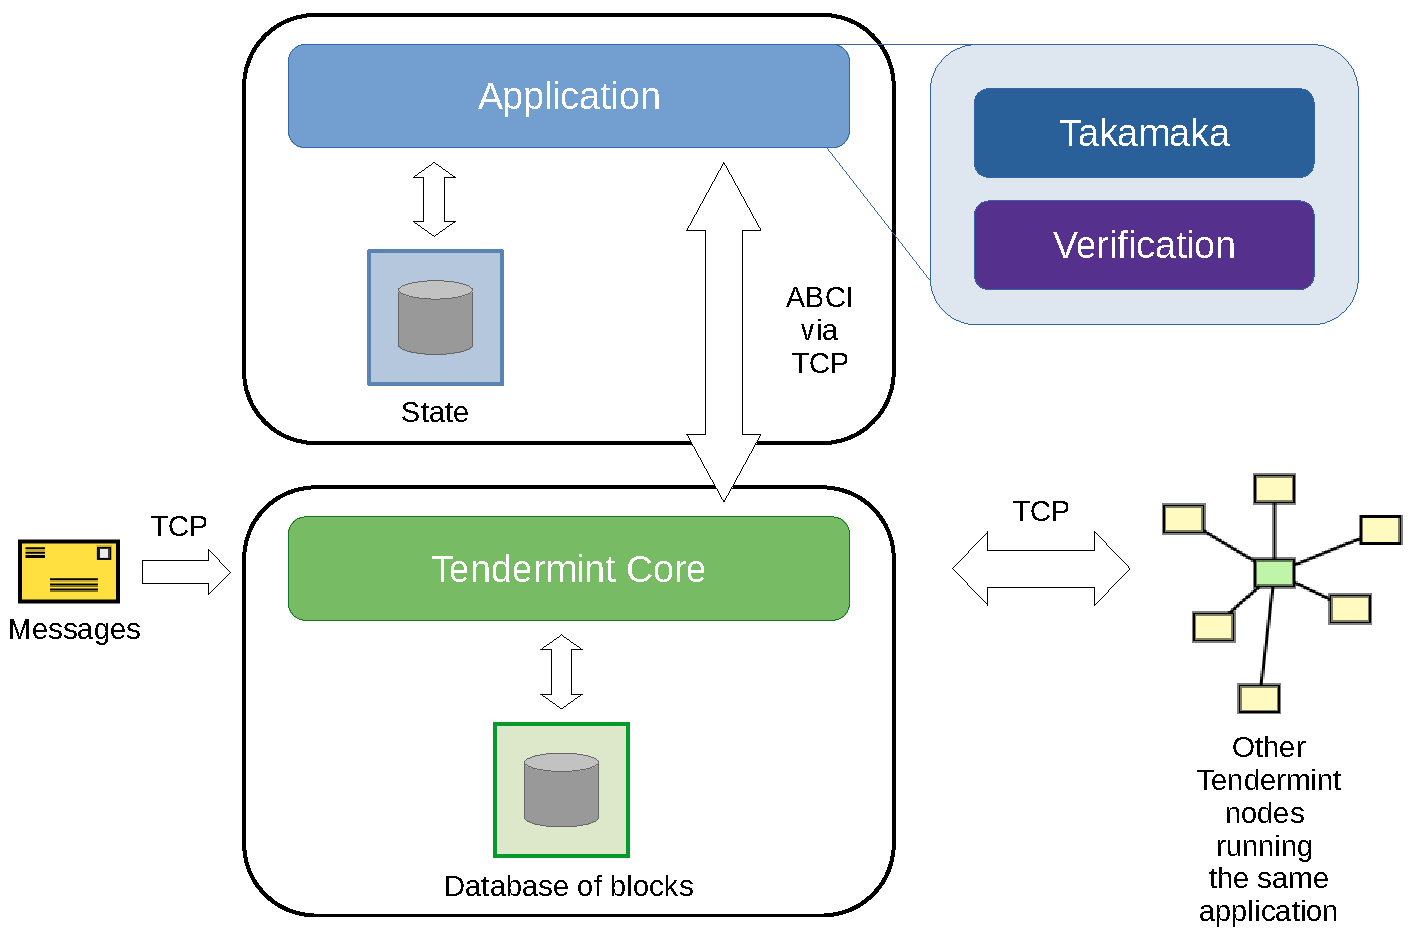
\includegraphics[scale=0.4]{pictures/architecture.pdf}
  \end{center}
  \caption{Architecture of our distributed application performing on-chain verification.}
  \label{fig:architecture}
\end{figure}

\bibliographystyle{plain}
\bibliography{biblio}

\end{document}
